\section{Our data as a platform for evaluation}

% The most immediate application for our corpus is in developing models for the task of NLI. In particular, since it is dramatically larger than any existing corpus of comparable quality, we expect it to be suitable for training  parameter-rich models like neural networks for this task. In this section, we explore the performance of a range of standard and novel models trained on the corpus.

\subsection{Standard entailment models}

The first class of models is from the Excitement Open
  Platform (EOP,
  \citealt{pado2014design,magnini2014excitement})---an open source platform for RTE research.
%  which
%  is distributed alongside a number of RTE pipelines.
We additionally evaluate against a strong but simple classifier-based model with
  both unlexicalized and lexicalized features.

%
% EOP
%
\paragraph{Excitement Open Platform}
% what is EOP
The Excitement Open Platform is a tool to quickly develop NLI systems
  while sharing components such as common lexical resources and 
  evaluation sets.
We evaluate against three algorithms included in the distribution,
  and also evaluated in \newcite{magnini2014excitement}.
These are: 
  (1) a simple edit-distance based algorithm; and
  (2) a classifier-based algorithm.
%  (3) an algorithm based around tree transformations.

%% 9 systems compared against
%A number of systems have been built using the platform, 9 of them
%  applicable to English are publicly distributed with version 1.2.1
%  of the software.
%% these fall into 2 classes
%These fall into two classes of algorithms: 2 are edit distance based,
%  whereas the remaining 7 make use of different features in a
%  maximum entropy classifier.
%
%%% methodology
%%We convert the 3-way classification task in SNLI into the RTE setting
%%  by labeling both the \unknown\ and \contradiction\
%%  labels as negative entailment, and treating the \entailment\ label as
%%  the positive entailment.
%%This creates a biased dataset of 66\% negative examples.
%% we report the best results from each class
%We run the top performing edit-distance based algorithm and the top
%  performing classifier-based algorithm on our test set, as
%  determined by performance on the development set.
%Note that these models were run using the default configuration
%  with minimal tuning.
%The results should therefore be taken as a strong baseline for
%  NLI-style approaches to the problem, rather than necessarily
%  representing the state-of-the-art system's performance on the
%  task.
%%We run each of the 9 algorithms distributed with EOP on the 2-class
%%  SNLI dataset, and report results for the best edit distance 
%%  configuration and the best classifier based configuration, as
%%  determined by performance on the development set.

%
% EOP RESULTS TABLE
%

% The table
\begin{table}
\begin{center}
\def\t#1{\small{#1}}
\begin{tabular}{l@{\hskip \colspaceL}c@{\hskip \colspaceL}c@{\hskip \colspaceL}c}
\toprule
\b{System} & \b{Our corpus} & \b{SICK} & \b{RTE-3} \\
\midrule
\t{Edit Distance Based}        & \t{71.9} & \t{65.4} & \b{61.9} \\
\t{Classifier Based}           & \b{72.2} & \b{71.4} & \t{61.5} \\
%\midrule
%\t{Classifier Based (3-class)} & \t{??.?} & \t{65.6} & \t{} \\
%\t{Transformation Based} & \t{36.0} & \t{76.7} & \t{56.4} \\  % broken! At least, on SNLI...
\bottomrule
\end{tabular}
\end{center}
% The caption
\caption{
\label{tab:eopresults}
2-class test accuracy for two systems included in the
  Excitement Open Platform.
%All RTE results are 2-class accuracy.
%The transformation-based model allows for 3-class predictions on our
%  corpus and SICK; these are reported in the last row.
}
\end{table}
%
% END EOP RESULTS TABLE
%

% the best systems
We report results in \reftab{tab:eopresults}, covering both our own test set,
  the SICK test data, and the standard RTE-3 test set \cite{giampiccolo2007third}.
Each of the models was trained on its own training set.
%The results for RTE-3 are taken from \newcite{magnini2014excitement}.
The edit distance and classifier based models are evaluated only on
  2-class entailment; all RTE results are likewise reported for 2-class entailment.
To convert 3-class problems like SICK and our corpus to this setting, all instances
  of \contradiction\ and \unknown\ are converted to nonentailment.
This yields a chance baseline accuracy of 66\% on our corpus, and 71\% on SICK.
We train these models without using any of the included lexical
  resources, so these results do not represent state-of-the-art
  RTE systems, but rather give an indication of the relative
  difficulties of the datasets.

%The best edit distance algorithm tunes the weight of the three 
%  case-insensitive edit distance operations on the training set, 
%  after removing stop words.
%The best classifier-based system makes use of information from
%  WordNet \cite{miller1995wordnet} and VerbOcean
%  \cite{chklovski2004verbocean}, and makes use of features
%  based on tree patterns and dependency tree skeletons
%  \cite{wang2007recognizing}.
%Unsurprisingly, the classification-based approach outperforms simple
%  edit distance metrics, and performs quite well despite relatively
%  little lexicalization.
%\todo{Is the RTE3 model trained on RTE3?}

%
% Lexicalized Classifier
%
\paragraph{Lexicalized Classifier}
Unlike the RTE datasets, our corpus's size supports approaches which make use of rich lexicalized features.
We evaluate a simple lexicalized classifier to explore the ability of non-specialized models to exploit these features in lieu of more involved language understanding.
Our classifier implements 6 feature types:
\begin{enumerate}
\setlength\itemsep{-0.25em}
  \item The BLEU score of the \hypothesis\ with respect
  to the \premise, using an n-gram length between 1 and 4.

  \item The length difference between the \hypothesis\ and the \premise, as a real-valued
  feature.

  \item The overlap between words in the \premise\ and \hypothesis,
  both as an absolute count and a percentage of possible overlap, and both over 
  all words and over just nouns, verbs, adjectives, 
  and adverbs.
  
  \item\label{lst:ngram} An indicator for every unigram and bigram in the \hypothesis.

  \item\label{lst:unigram} Cross-unigrams: for every pair of words across the \premise\ and \hypothesis\ which share a 
  POS tag, an indicator feature over the two words.
  
  \item\label{lst:bigram} Cross-bigrams: for every pair of bigrams across the \premise\ and \hypothesis\ which share a 
  POS tag on the second word, an indicator feature over the two bigrams.
\end{enumerate}

%
% BOW RESULTS TABLE
%

% The table
\begin{table}
\begin{center}
\begin{tabular}{l@{\hskip \colspaceL}c@{\hskip \colspaceS}c@{\hskip \colspaceL}c}
\toprule
\b{System}	 & \multicolumn{2}{c}{\hspace{-1.2em}\b{Our corpus}} & \b{SICK}\\
 & \t{Train} & \t{Test} & \t{Test}\\
\midrule
\t{Lexicalized}            & \t{99.7}  & \b{78.2} & \b{77.3} \\ % & \t{78.7}
\t{Unigrams Only}          & \t{93.1} & \t{71.6} & \t{74.0} \\ % & \t{72.2}
\t{Unlexicalized}          & \t{49.4} & \t{50.4} & \t{69.4}\\ % & \t{50.1} % Last value was 50.39; rounded for consistency.
\bottomrule
\end{tabular}
\end{center}
% The caption
\caption{
\label{tab:bowresults}
3-class accuracy, training and testing on either our data or SICK, including models lacking cross-bigram features 
  (Feature \ref{lst:bigram}), and lacking all lexical
  features (Features \ref{lst:ngram}--\ref{lst:bigram}).
}
\end{table}
%
% END BOW RESULTS TABLE
%


% Results
We report results in \reftab{tab:bowresults}, along with ablation studies for removing
  the cross-bigram features (leaving only the cross-unigram feature),
  and for removing all lexicalized features.
% Insights 1: lexicalization helps a bunch
On our large corpus in particular, there is a substantial jump in accuracy from using
  lexicalized features, and another from using the very sparse
  cross-bigram features.
The latter  result can be explained if
  the classifier automatically learns to recognize explicit negations and adjective
  modification, and a similar result was shown in
  \newcite{sidaw12simple} for bigram features in sentiment analysis.
  
% Insight 2: do well without alignments
Another surprising fact is that the classifier performs as well as it
  does without any notion of alignment or tree transformations.
Although we expect that richer models would perform better,
  the results suggest that given enough data, cross bigrams with the noisy 
  part-of-speech overlap constraint can produce an effective model.

%In fact, the addition of these features alone allow the classifier to
%  outperform many of the .
%  This seems initially surprising, but it makes sense given how our corpus differs from existing ones:
%  the EOP systems have been tuned on relatively small corpora
%  ($\approx$1600 examples), whereas a classifier trained on our corpus can make use of
%  over two orders of magnitude more data.

\subsection{Sentence embeddings and NLI}\label{sentence-embedding}

Our corpus is suitably large and diverse to make it possible to train neural network models that produce distributed representations of sentence meaning. In this section, we compare the performance of three such models on the corpus. To focus specifically on the strengths of these models at producing informative sentence representations, we use sentence embedding as an intermediate step in the NLI classification task: each model must produce a vector representation of each of the two sentences without using any context from the other sentence, and the two resulting vectors are then passed to a neural network classifier which predicts the label for the pair. This choice allows us to focus on existing models for sentence embedding, and it allows us to evaluate the ability of those models to learn useful representations of meaning (which may be independently useful for subsequent tasks), at the cost of excluding from consideration possible strong neural models for NLI that directly compare the two inputs at the word or phrase level.


\begin{figure}[tp]
  \centering
\scalebox{0.85}{
 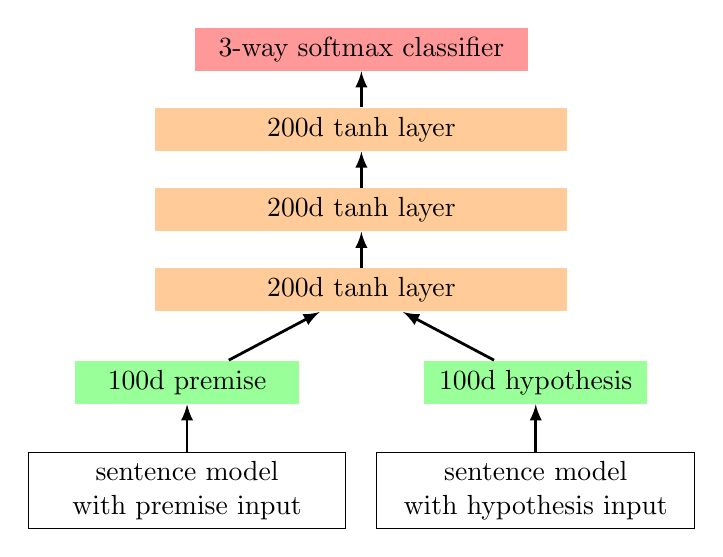
\begin{tikzpicture}
    \def\dx{21pt}
    \def\dy{29pt}

    \tikzstyle{label}=[text width=40mm,align=center]    
    \tikzstyle{softmax}=[fill=red!40,text width=40mm,align=center]
    \tikzstyle{preclass}=[fill=orange!40,text width=50mm,align=center]
    \tikzstyle{e}=[fill=green!40,text width=26mm,align=center]
    \tikzstyle{m}=[draw=black,text width=38mm,align=center]    
    
    \node[softmax]  (softmax) at (0*\dx,6*\dy) {3-way softmax classifier};
    \node[preclass]  (pc3) at (0*\dx,5*\dy) {200d $\tanh$ layer};
    \node[preclass]  (pc2) at (0*\dx,4*\dy) {200d $\tanh$ layer};
    \node[preclass]  (pc1) at (0*\dx,3*\dy) {200d $\tanh$ layer};
    \node[e]  (pe) at (-3*\dx,1.85*\dy) {100d premise};
    \node[e]  (he) at (3*\dx,1.85*\dy) {100d hypothesis};
    \node[m]  (pem) at (-3*\dx,0.5*\dy) {sentence model\\ with premise input};
    \node[m]  (hem) at (3*\dx,0.5*\dy) {sentence model\\ with hypothesis input};    
    
    \pgfsetarrowsend{latex}
    \tikzstyle{fwd} = [draw=black, line width=1pt]

          \draw [fwd] (pc3) -- (softmax);
          \draw [fwd] (pc2) -- (pc3);
          \draw [fwd] (pc1) -- (pc2);
          \draw [fwd] (pe) -- (pc1);
          \draw [fwd] (he) -- (pc1);
          \draw [fwd] (hem) -- (he);
          \draw [fwd] (pem) -- (pe);

  \end{tikzpicture}}
	
        \caption{The neural network classification architecture: for each sentence embedding model evaluated in \reftabs{tab:nnresults}{tab:transferresults}, two identical copies of the model are run with the two sentences as input, and their outputs are used as the two 100d inputs shown here.}
  \label{modelstructure}
\end{figure}

Our neural network classifier, depicted in \reffig{modelstructure} (and based on a one-layer model in \citealt{Bowman:Potts:Manning:2014}), is simply a stack of three 200d $\tanh$ layers, with the bottom layer taking the concatenated sentence representations as input and the top layer feeding a softmax classifier, all trained jointly with the sentence embedding model itself.

We test three sentence embedding models, each set to use 100d phrase and sentence embeddings. Our baseline sentence embedding model simply sums the embeddings of the words in each sentence. In addition, we experiment with two simple sequence embedding models: a plain RNN and an LSTM RNN \cite{hochreiter1997long}. Both use the simple conventional layout with one layer per input token.

The word embeddings for all of the models are initialized with the 300d reference GloVe vectors (840B token version, \citealt{pennington2014glove}) and fine-tuned as part of training. In addition, all of the models use an additional $\tanh$ neural network layer to map these 300d embeddings into the lower-dimensional phrase and sentence embedding space. All of the models are randomly initialized using standard techniques and trained using AdaDelta \cite{zeiler2012adadelta} minibatch SGD until performance on the development set stops improving. We applied L2 regularization to all models, manually tuning the strength coefficient $\lambda$ for each, and additionally applied dropout \cite{srivastava2014dropout} to the inputs and outputs of the sentence embedding models (though not to its internal connections) with a fixed dropout rate. All models were implemented in a common framework for this paper, and the implementations will be made available at publication time.

\begin{table}
\begin{center}
\begin{tabular}{l@{\hskip \colspaceL}@{\hskip \colspaceL}c@{\hskip \colspaceL}c}
\toprule
\textbf{Sentence model} & \b{Train}  & \b{Test}\\
\midrule
\t{100d Sum of words}            & \t{79.3} & \t{75.3} \\
% scr/snlirc3d-snlirc3-only-l0.0001-dim100-ed300-td3-pen200-do0.9-0.9-co3-comp-1-dp1-gc5-lstminit5/stat_log
% 290500, dev 76.4, converged

\t{100d RNN}            & \t{73.1} & \t{72.2} \\	
% scr/snlirc3d-snlirc3-only-l0.0001-dim100-ed300-td3-pen200-do0.9-0.9-co3-comp3-dp1-gc5-lstminit5/stat_log
% 338500, dev 72.5, mostly converged

\t{100d LSTM RNN}            & \t{84.8} & \b{77.6} \\
% scr/snlirc3d-snlirc3-only-l3e-05-dim100-ed300-td3-pen200-do0.95-0.95-co3-comp2-dp1-gc5-lstminit5/stat_log
% 372000, dev 79.11, mostly converged

% \t{100d TreeRNN}            & \t{69?} & \t{69?} \\
% \t{50d TreeRNTN}            & \t{61?} & \t{60?} \\
% \t{100d LSTM TreeRNN}            & \t{72?} & \t{73?} \\
\bottomrule
\end{tabular}
\end{center}
% The caption
\caption{
\label{tab:nnresults}
Accuracy in 3-class classification on our training and test sets for each model.
}
\end{table}

The results are shown in \reftab{tab:nnresults}. The sum of words model performed slightly worse than the fundamentally similar lexicalized classifier---while the sum of words model is able to use pretrained word embeddings to better handle rare words, it lacks even the rudimentary sensitivity to word order that the lexicalized model's bigram features provide. Of the two RNN models, the LSTM's more robust ability to learn long-term dependencies serves it well, giving it a substantial advantage over the plain RNN, and  resulting in performance that is essentially equivalent to the lexicalized classifier on the test set (LSTM performance near the stopping iteration varies by up to 0.5\% between evaluation steps). While the lexicalized model fits the test set perfectly, the gap between train and test set accuracy is relatively small for all three neural network models, suggesting that research into significantly higher capacity versions of these models could be productive.

\subsection{Analysis and discussion}

\Reffig{fig:bowlearncurve} shows a learning curve for the LSTM and the lexicalized and unlexicalized feature-based models. This learning curve shows that the large size of the corpus is crucial to both the LSTM and the lexicalized model, and suggests that additional data would yield still better performance for both. In addition, though the LSTM and the lexicalized model show similar performance when trained on the current full corpus, the steeper slope for the LSTM suggests that its ability to learn arbitrarily structured representations of sentence meaning would give it an advantage over the more constrained lexicalized model on still larger datasets.

% useful resource in the development of more sophisticated SE models

\Fig{learning_curves_bow.pdf}{0.45}{bowlearncurve}{
A learning curve for the lexicalized and unlexicalized baseline classifiers and the LSTM,
plotted on a log scale. The y-axis starts at a random-chance accuracy of 33\%. The minibatch size of 64 that we used to tune the LSTM sets a lower bound on data for that model.}

% Insights 2: the learning curve for the unlexicalized classifier is sad
We were struck by the speed with which the lexicalized classifier outperforms its unlexicalized counterpart.
With only 100 training examples, the cross-bigram classifier is already performing better.
Empirically, we find that the top weighted features for the classifier
  trained on 100 examples tend to be high precision entailments;
  e.g.,
  \textit{playing} $\rightarrow$ \textit{outside}
  (most scenes are outdoors), \textit{a banana} $\rightarrow$
  \textit{person eating}.
If relatively few spurious entailments get high weight---as it appears
is the case---then it makes sense that, when these do fire, they
boost accuracy in identifying entailments.
  
There are revealing patterns in the errors common to all the models
considered here. Despite the large size of the training corpus and the
distributional information captured by GloVe initialization, many
lexical relationships are still misanalyzed, leading to incorrect
predictions of \ii{independent}, even for pairs that are common in the
training corpus like \word{beach}/\word{surf} and
\word{sprinter}/\word{runner}. Semantic mistakes at the phrasal level
(e.g., predicting contradiction for \word{A male is placing an order in a 
deli}/\word{A man buying a sandwich at a deli}) indicate
that additional attention to compositional semantics would pay off.
%
% Others that could replace the above:
% \word{Two teen girls relax on a black futon}/\word{Two young girls are sitting inside}
% \word{A male is placing an order in a deli}/\word{A man buying a sandwich at a deli}
% \word{A shopper buys cat food at a Walmart}/\word{A person shops for their pet at a store}
However, many of the persistent problems run deeper, to inferences
that depend on world knowledge and context-specific inferences, as in
the entailment pair \word{A race car driver leaps from a burning
  car}/\word{A race car driver escaping danger}, for which both
the lexicalized classifier and the LSTM predict \ii{neutral}. 
In other cases, the models' attempts to shortcut this kind of inference 
through lexical cues can lead them astray. 
Some of these examples have qualities
reminiscent of Winograd schemas \cite{Winograd:1972,Levesque:2013}. For
example, all the models wrongly predict
entailment for \word{A young girl throws sand toward the
  ocean}/\word{A girl can't stand the ocean}, presumably because of
distributional associations between \word{throws} and \word{can't
  stand}.

Analysis of the models' predictions also yields insights into the
extent to which they grapple with event and entity coreference. For
the most part, the original image prompts contained a focal element
that the caption writer identified with a syntactic subject, following
information structuring conventions associating subjects and topics in
English \cite{Ward04}. Our annotators generally followed suit, writing
sentences that, while structurally diverse, share topic/focus (theme/rheme)
structure with their premises.
This promotes a coherent, situation-specific construal of each sentence
pair. This is information that our models can easily take advantage
of, but it can lead them astray. For instance, all of them stumble
with the amusingly simple case \emph{A woman prepares ingredients for
  a bowl of soup}/\emph{A soup bowl prepares a woman}, in which prior
expectations about parallelism are not met. Another headline example
of this type is \emph{A man wearing padded arm protection is being
  bitten by a German shepherd dog}/\emph{A man bit a dog}, which all
the models wrongly diagnose as \ii{entailment}, though the sentences
report two very different stories.

\section{Transfer learning with SICK}

To the extent that successfully training a neural network model like our LSTM on our corpus forces that model to encode broadly accurate representations of English scene descriptions and to build an entailment classifier over those relations, we should expect it to be readily possible to adapt the trained model for use on other NLI tasks. In this section, we evaluate on the SICK entailment task using a simple transfer learning method and achieve competitive results.

\begin{table}
\begin{center}
\begin{tabular}{l@{\hskip \colspaceL}@{\hskip \colspaceL}c@{\hskip \colspaceL}c}
\toprule
\textbf{Training sets} & \b{Train}  & \b{Test}\\
\midrule
\t{Our data only}            & \t{42.0} & \t{46.7} \\
% scr/transfer5-sick-only-transfer-l0.0001-dim100-ed300-td3-pen200-do0.95-0.95-ws3-adi1-comp2-cdim1/stat_log
% Step 0, no learning intended after transfer
\t{SICK only}            & \t{100} & \t{71.3} \\
% From: ~/quant/transfer-sick-only-l0.0001-dim50-ed200-td3-pen100-do0.9-0.9-ws1-par0-comp2-cdim1/
\t{Our data and SICK (transfer)}            & \t{99.9} & \b{80.8} \\
% From: ~/quant/transfer5-sick-only-transfer-l0.0001-dim100-ed300-td3-pen200-do0.95-0.95-ws3-adi0-comp2-cdim1/stat_log
\bottomrule
\end{tabular}
\end{center}

\caption{\label{tab:transferresults}
LSTM 3-class accuracy on the SICK train and test sets under three training regimes.} 
\end{table}


To perform transfer, we take the parameters of the LSTM RNN model trained on our corpus and use them to initialize a new model, which is trained from that point only on the training portion of SICK. The only newly initialized parameters are softmax layer parameters and the embeddings for words that appear in SICK, but not in our corpus (which are populated with GloVe embeddings as above). We use the same model hyperparameters that were used to train the original model, with the exception of the L2 regularization strength, which is re-tuned. We additionally transfer the accumulators that are used by AdaDelta to set the learning rates. This lowers the starting learning rates, and is intended to ensure that the model does not learn too quickly in its first few epochs after transfer and destroy the knowledge accumulated in the pre-transfer phase of training. We tune the regularization parameter separately for each case. 

The results are shown in \reftab{tab:transferresults}. Training on SICK alone yields poor performance, and the model trained on our data misunderstands the subtly different meanings of the (identically named) SICK labels, labeling more \ii{neutral} examples as \ii{contradiction}s than correctly. Transferring representations, in contrast, yields the best performance yet reported on SICK for an unaugmented neural network model, surpasses the available EOP models, and approaches both the overall state of the art at 84.6\% \cite{lai2014illinois} and the 84\% level of interannotator agreement, which likely represents an approximate performance ceiling. This suggests that the introduction of a large high-quality corpus makes it  possible to train representation-learning models for sentence meaning that are competitive with the best hand-engineered models on inference tasks.

We attempted to apply this same transfer evaluation technique to the RTE-3 challenge, but found that the small training set (800 examples) did not allow the model to adapt to the unfamiliar genre of text used in that corpus, such that no training configuration yielded competitive performance.
Further research on effective transfer learning on small data sets with neural models might facilitate improvements here.


% A woman prepares ingredients for a bowl of soup.	A soup bowl prepares a woman.

